% ============================================================
%  CHAPTER 1: INTRODUCTION
% ============================================================
\chapter{Introduction}

This chapter provides an overview of the problem addressed in this project.
Section~1.1 introduces the supply chain management domain and discusses the
background, the problem being solved, the proposed solution, and the expected
outcomes. Section~1.2 lists the specific technical contributions made through
this work. Section~1.3 outlines how the remainder of the thesis is organized.

% ================================================================
\section{Supply Chain Management}

% ----------------------------------------------------------------
\subsection{Background}

The supply chain is the sequence of processes through which raw materials are
sourced, processed, and delivered as finished goods to end consumers. In the
context of fast-moving consumer goods (FMCG), this chain typically spans
manufacturers, regional distribution hubs, city-level warehouses, and retail
outlets. Effective management of this chain directly affects product availability,
operational costs, and customer satisfaction. Traditional supply chain management
(SCM) relied primarily on deterministic models, fixed routing schedules, and
rule-based reorder policies. These approaches performed adequately when demand
was stable and supply was predictable.

India presents a particularly challenging environment for supply chain management.
The rapid growth of e-commerce, the expansion of cold-chain logistics for
perishable goods, and the diversity of urban road networks have made static
routing policies increasingly inadequate. Tier-2 cities such as Nagpur represent
a critical and growing segment of this logistics challenge. Nagpur serves as a
major road and rail junction in central India, making it a significant node in
distribution networks that cover Maharashtra and the surrounding states. Its road
network spans multiple distinct zones, including residential neighborhoods with
high residential traffic density, commercial office corridors, shopping and market
districts, and high-speed highway bypasses. Each of these zones exhibits a
different traffic profile depending on the time of day and the day of the week,
making static routing ineffective even within a single city.

The problem is compounded when cargo has a limited shelf life. Perishable goods
such as dairy products, medicines, and fresh produce carry a Remaining Shelf Life
(RSL) that decreases with every hour of transit. A truck that takes a slightly
longer but less congested route may arrive on time, while a truck that follows the
shortest path through a congested market zone may arrive with cargo that has
deteriorated significantly. Simultaneously, fleet operators face pressure to
minimize fuel consumption, since fuel costs represent a major portion of logistics
expenses. These competing constraints, namely freshness, speed, fuel efficiency,
and road safety, cannot be balanced simultaneously by any single static rule. This
motivates the use of artificial intelligence to make adaptive, real-time routing
decisions.

% ----------------------------------------------------------------
\subsection{Problem Statement}

The core problem addressed in this project is the dynamic routing of a delivery
fleet under multiple competing real-time constraints in an urban logistics network.
The specific challenges are as follows.

First, delivery routes must respond to conditions that change continuously: road
accidents, unexpected weather events such as monsoon rainfall, and fluctuating
traffic density across different zones and times of day. A route that is optimal
at 9~AM may be severely suboptimal by 11~AM once office-hour congestion sets in.

Second, cargo freshness imposes a time-based deadline on each delivery. Once a
batch of goods is loaded onto a truck, the RSL begins declining. The routing
system must factor in how much freshness a cargo will have remaining when it
reaches the retailer, not just how quickly the truck will physically arrive.

Third, fuel consumption is a direct cost. Routing the entire fleet aggressively
for speed maximizes throughput but depletes fuel faster, increases refueling
frequency, and raises operational costs. A purely fuel-conservative strategy, on
the other hand, results in slower deliveries and more stockouts at retailer outlets.

Fourth, current heuristic routing algorithms such as A* use a single fixed cost
function and cannot switch between optimization objectives based on the current
state of the fleet. A truck that is almost out of fuel should be routed
conservatively, while a truck carrying cargo with a short remaining shelf life
should be routed aggressively for speed. No single static heuristic can capture
this context-sensitive decision-making requirement.

% ----------------------------------------------------------------
\subsection{Solution}

This project proposes a Supply Chain Digital Twin for the city of Nagpur,
implemented as a discrete-event simulation environment in which a fleet of
delivery trucks operates over a realistic road network, subject to dynamic
weather, traffic, and accident events. The Digital Twin serves as a safe,
repeatable environment for training and validating artificial intelligence models
before deployment.

The routing intelligence of the system is organized into a three-tier hierarchy.
The first tier is a Central PPO Brain, a Proximal Policy Optimization (PPO) agent
trained offline to observe the state of the full fleet and select a macro-level
routing strategy from three options: Fuel-Priority, RSL-Priority, or
Speed-Priority. The second tier is an Edge Q-Learning Agent embedded within each
individual truck, which performs micro-level emergency rerouting in real time when
sudden events such as accidents or extreme weather block the current route. The
third tier is an ETA Forecaster based on online Ridge Regression, which predicts
travel time for individual road segments based on real-time conditions including
the zone, time of day, day of the week, weather, and traffic density. This
prediction feeds directly into the route planner's cost function, improving the
accuracy of route selection.

\begin{figure}[h!]
    \centering
    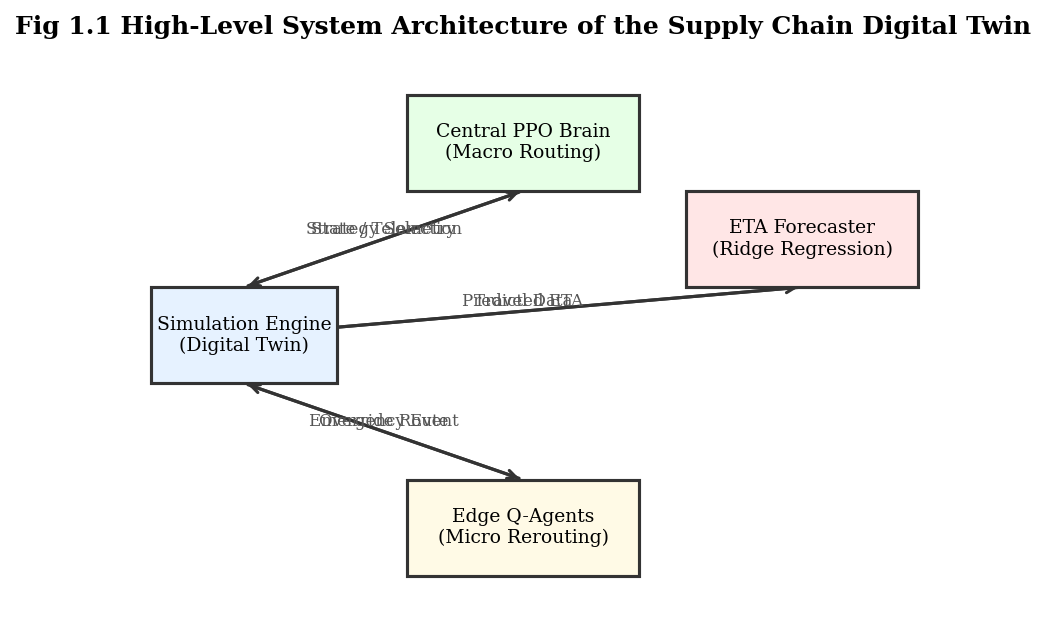
\includegraphics[width=0.95\textwidth]{images/fig1_1_system_overview.png}
    \caption{High-Level System Architecture of the Supply Chain Digital Twin}
    \label{fig:system_overview}
\end{figure}

Figure~\ref{fig:system_overview} shows how these components interact. Orders are
placed by retailer nodes and processed by the simulation engine. The Central PPO
Brain observes the 25-dimensional fleet state and selects a strategy. The ETA
Forecaster continuously refines its travel time estimates. The Edge Agents handle
unexpected disruptions. Together, these three tiers enable the fleet to make
intelligent, context-sensitive routing decisions across the full year of operation.

% ----------------------------------------------------------------
\subsection{Outcomes}

The system was validated through a 365-day comparative simulation benchmark, with
both the baseline heuristic router and the full AI-enabled system run under
identical conditions. The following outcomes were observed from the results.

\begin{itemize}
    \item The AI-enabled system fulfilled 323 additional orders compared to the
    baseline over the full year, an increase of 4.7\%.
    \item Total cargo delivered increased by 474,707~kg, representing nearly half
    a million additional kilograms of goods reaching retailers.
    \item Retailer stockout events were reduced from 70,898 to 33,401, a reduction
    of 52.9\%, demonstrating substantially improved supply continuity.
    \item Road accidents were reduced from 2,212 to 2,077, showing that the AI
    learned to prefer safer routing patterns without being explicitly instructed to.
    \item Cargo freshness at the point of delivery averaged 99.7\% in both the
    baseline and RL configurations, confirming that RSL was preserved throughout
    transit and not sacrificed for throughput.
    \item Fuel efficiency remained identical between the two configurations at
    78.7\%, proving that the throughput gains were achieved without any additional
    fuel cost.
\end{itemize}

% ================================================================
\section{Contribution}

The specific technical contributions of this project are listed below.

\begin{itemize}
    \item \textbf{Supply Chain Digital Twin Simulation Engine:} A complete
    discrete-event simulation of the Nagpur city logistics network was designed and
    implemented. The simulation models a multi-zone road graph, a fleet of delivery
    trucks, warehouse and retailer nodes, and dynamic environmental events including
    weather, traffic density, and road accidents. This engine serves as the training
    and evaluation environment for all AI components.

    \item \textbf{Central PPO Routing Agent:} A Proximal Policy Optimization agent
    was designed, trained for 50,000 steps, and deployed for macro-level strategy
    selection. The agent observes a 25-dimensional state vector and selects one of
    three routing strategies per dispatch cycle.

    \item \textbf{Edge Q-Learning Emergency Override Agent:} A per-truck tabular
    Q-Learning agent was designed for real-time emergency micro-rerouting. The agent
    operates entirely online, updating its Q-table after each emergency event, and
    can override the Central Brain's strategy when local road conditions make it
    dangerous or infeasible.

    \item \textbf{8-Dimensional Spatial-Temporal ETA Forecaster:} An online Ridge
    Regression model was designed and integrated to predict travel time for each road
    segment. The feature vector was upgraded from a 5-dimensional baseline to an
    8-dimensional vector incorporating circular time-of-day encoding, circular
    day-of-week encoding, and geographic zone classification. This allows the
    forecaster to capture temporal and spatial traffic patterns simultaneously.

    \item \textbf{Reward Normalization Framework (5:1 Ratio):} A mathematical
    analysis of the physical magnitudes of fuel consumption and cargo decay rates was
    used to derive a 5-to-1 normalization ratio for the PPO reward function. This
    normalization prevents the PPO agent from defaulting to a single objective and
    enables true dynamic strategy switching.

    \item \textbf{Anti-Thrashing GPS State Lock:} A route-thrashing bug was
    identified and resolved through the implementation of a state machine lock inside
    the truck agent. This fix was critical: without it, the fleet delivery rate
    collapsed to 49.8\% due to constant route recalculation.

    \item \textbf{365-Day Long-Term Validation Benchmark:} The system was validated
    over a full simulated year (365 days) under a fixed reproducible seed, producing
    a statistically meaningful comparison between the baseline heuristic router and
    the full AI-enabled system.
\end{itemize}

% ================================================================
\section{Organization of Thesis}

This thesis is organized to systematically cover all aspects of the proposed
system, from motivation through implementation and results.

Chapter 1 introduces the problem, the solution approach, and the specific
technical contributions. Chapter 2 reviews the existing literature on traditional
routing methods, machine learning in logistics, and the theoretical foundations of
reinforcement learning. Chapter 3 describes the data generated by the simulation
environment and how it is preprocessed into state representations for the AI
models. Chapter 4 presents the full design and implementation of all system
components, including the simulation engine, the three-tier AI architecture, and
the training procedure. Chapter 5 presents and analyzes the results from the
365-day benchmark. Chapter 6 concludes the thesis and discusses directions for
future work. References are listed in Chapter 7 in IEEE numbered format.

% ================================================================
\vspace{1cm}
\noindent \textbf{Chapter Summary:} This chapter introduced the problem of dynamic
fleet routing under competing real-time constraints in the Nagpur city supply chain.
The proposed solution, a three-tier AI architecture embedded within a Digital Twin
simulation environment, was outlined, and the specific contributions of this project
were enumerated. The next chapter reviews the existing literature on routing methods
and reinforcement learning techniques that form the theoretical basis of this work.
